%\documentclass[preprint,authoryear,12pt]{elsarticle}
\documentclass[final,authoryear,5pt,times,twocolumn]{elsarticle}

\usepackage{tikz}
\usepackage{pgfplots}
\pgfrealjobname{article}
%TODO - remove \usepackage (convert images to pdf/eps)

\usepackage{amssymb}
\usepackage{amsmath}
\usepackage{booktabs}
\usepackage{textcomp}

\newcommand{\vect}[1] %vector notation
{{\bf {#1}}}
\newcommand{\npoly}{$n$-polytope}
\newcommand{\citepp}[4] %double parenthesis cite
{(\citealp[{#1}]{{#2}}; \citealp[{#3}]{{#4}})}
\newcommand{\bpm}{\begin{pmatrix}} %for matrix notation
\newcommand{\epm}{\end{pmatrix}}

\journal{Journal of Process Control}

\begin{document}

%% ==== HEAD ====
\begin{frontmatter}

\title{A Systematic Approach to Model Predictive Controller Constraint Handling: Rigorous Geometric Methods}

\author{Andr\'e H. Campher}
\ead{ahcampher@tuks.co.za}

\author{Carl Sandrock\corref{cor1}}
\ead{carl.sandrock@up.ac.za}

\cortext[cor1]{Corresponding author\\Tel.: +27 12 420 2197; Fax: +27 12 420 5048}

\address{Department of Chemical Engineering, University of Pretoria, Pretoria, 0001, South Africa}

\begin{abstract}
The models used by model predictive controllers (MPCs) to predict future outcomes are usually unconstrained forms like impulse or step responses and discrete state space models. 
Certain MPC algorithms allow constraints  to be imposed on the inputs or outputs of a system; but they may be infeasible as they are not checked for consistency via the process model. 
Consistent constraint handling methods -- which account for their interdependence and disambiguate the language used to specify constraints -- would therefore be an attractive addition to any MPC package.

A rigorous and systematic approach to constraint management is proposed, building on the work of \citet{vinsonartoi} in interpreting constraint interactions. 
The method focuses on linear steady-state system models, and provides routines to obtain the following information: effects of constraint changes on the corresponding input or output constraints, feasibility checks for constraints and constraint-type information.

Mathematical rigour and unambiguous language for identifying constraint types were key design criteria. 
The application of the method is illustrated for a laboratory scale distillation column running commercial MPC packages.
\end{abstract}

\begin{keyword}
constraint handling \sep model predictive control \sep geometric methods \sep operability index
\end{keyword}

\end{frontmatter}

%\linenumbers


%% ==== BODY ====
\section{Introduction}\label{sec:intro}
Model predictive controllers use process models to predict the effect of the inputs of a system on its outputs.
The ability of some MPC algorithms to impose constraints on the outputs or inputs is one of their biggest selling points.
These constraints are also interdependent via the process model.

At present, commercial MPC packages only validate constraints against high and low limits set by external engineering criteria that are not based on the process model.
This gives rise to the following problems, both of which could result in infeasible controllers and unrealistic control expectations:
\begin{itemize}
  \item Specified constraints on an input or output may be infeasible due to their corresponding output or input requirements.
  \item Changing of constraints and the possible clamping of corresponding outputs or inputs are not evident (or quantified).
\end{itemize}

This paper proposes a method of systematically managing constraints imposed on MPCs, determining feasible constraints and reformatting them to be directly implemented in commercial MPC structures.
Building on the work by \citet{vinsonartoi}, \citet{opconproc} and \citet{limaphd} on constraint interaction, a method like this would help avoid infeasible constraints and further the understanding of constraint interaction in MPCs.

Mathematical rigour and unambiguous language when specifying constraints were key design criteria.
Linear steady-state models are considered along with linear constraints on the inputs and outputs.
This paper will therefore focus only on convex sets in the input and output space.


\section{Background}\label{sec:background}
\subsection{Mathematical Preliminaries}
A few of the mathematical concepts on which the proposed method relies are briefly reviewed in this section.

\subsubsection{Convex geometry}
A half-space is defined as the section of an $n$-dimensional space lying on one side of an ($n-1$)-dimensional hyperplane \citep[1282]{crcmaths}.

The following nomenclature is adopted, following \citet[487]{bayerlee};
\begin{itemize}
\item polytope - the intersection of closed half-spaces in $\mathbb{R}^n$.
A polytope of $n$ dimensions will simply be referred to as an $n$-polytope.
\item vertex - a 0 dimensional face of an \npoly.
\item facet - an $n-1$ dimensional face of an \npoly.
\end{itemize}

Linear constraints (as described in equation~\ref{eq:gencons}) are equivalent to half-spaces in $\mathbb{R}^n$ in both their mathematical description and meaning.
From this we can conclude that all polytopes generated by linear constraints (half-spaces) are convex, as they have supporting hyperplanes at each boundary point \citep[21]{manilev}.
From this it also follows that the intersection of such convex polytopes will be convex.
This is due to the resulting intersection being merely a subset of the half-spaces defining the two intersecting polytopes.

\subsubsection{Constraint Formulation}
Constraints on the inputs ($\vect{u}$) or outputs ($\vect{y}$) of a system can be represented as sets of inequalities.
For the most general linear case, they can be expressed as follows;
\begin{align}
  \label{eq:gencons}
  A_u\vect{u}_k &\leq b_u \\ \notag
  A_y\vect{y}_k &\leq b_y \\ \notag
\end{align}
where $A_u$ and $A_y$ are coefficient matrices, and $b_u$ and $b_y$  the half-space offsets.

For constraints on the rate of change of inputs, the formulation is similar to equation~\ref{eq:gencons}.
The change in $\vect{u}_k$ during a sampling instance is now considered thus;
\begin{align*}
  A_{\Delta u}\Delta \vect{u}_k &\leq b_{\Delta u} \notag \\
  \text{and}~~ \Delta \vect{u}_k &= \vect{u}_{k+1}-\vect{u}_k
\end{align*}

\subsubsection{Convex hull}
The convex hull or facet enumeration is used extensively for calculations in this project.
It is defined as the smallest convex set containing $P$ if $P$ is a set of points ($P \subseteq \mathbb{R}^n$) \citep[74]{wenger}.
In this paper, $P$ is constructed from a set of half-spaces resulting in a convex polytope.
For this reason the convex hull of $P$ and the half-spaces used to generate $P$ are equivalent.

\subsubsection{Process models}
The steady-state model of a linear system is the gain-matrix.
This is simply a matrix of constants in $\mathbb{R}$.
With this model matrix, obtaining the output space from the input space is a linear transformation \citep[48-49,~166]{leung} corresponding to a matrix multiplication of the vertices of the input space and the process model matrix.
This same property holds when transforming back to the input space from the output space.

Using linear models, the surface (or boundary) of the input space (a polytope) maps directly to the surface of the output space.
For this reason, the constraints specifying the input space can be used to generate the output space with full mathematical rigour.

Since the process model (gain-matrix) operates on, and outputs, deviation variables, a steady-state offset is added to produce absolute values.
This offset is calculated from the center of the input space and corresponds to the nominal point at which the process model is linearised.

\subsection{Model Predictive Control}
Since its successful implementation in the petrochemical industry, model predictive control (MPC) has gained widespread acceptance in the processing sector \citep[1]{maciejowskimpc}. 
This has led to the development of many commercial MPC packages such as DMCplus$^{\copyright}$ (Aspentech), RMPCT$^{\copyright}$ (Honeywell), Connoisseur$^{\copyright}$ (Invensys) and SMOC$^{\copyright}$ (Shell Global Solutions) \citep{qinbadgwell}.

The correct choice of model is one of the most important steps in the operation of MPCs \citep[17]{rossiter}.
This is due to the active use of the model in making predictions as the controller runs, and not serving merely as an analysis aid \citep[37]{maciejowskimpc}.

\subsubsection{Constraints}\label{sec:mpccons}
Most commercial MPC packages allow only high and low limits to be imposed on outputs or inputs.
The only validation of these constraints is against an outermost constraint set, often referred to as 'Engineering Limits'.
This set typically consists of physical limits on inputs and outputs, as well as limits that avoid damage to equipment.

\subsection{Process Operability}
Process operability is defined as ``the ease with which a process can be operated and controlled'' \citep[778]{marlin}.
Most process operability measures, however, are merely qualitative \citep[164]{skogestad}.

Both steady-state and dynamic operability measures exist and are used.
Since the operability index of \citet{vinsonartoi} focuses on input-output relationships rather than a system's dynamic states, the most common steady-state process operability techniques are briefly reviewed below.
\citet{vinsonphd} lists common dynamic operability measures and discuss their shortcomings in detail.

\subsubsection{Overview}
%1966
The relative gain array (RGA) is one of the most used operability measures \citep[576]{luyben} and relates input and output interactivity.
Each element in the RGA ($\beta_{ij}$) is defined as the ratio of the steady-state gain ratios between input, $i$, and output, $j$, when all other inputs and outputs are constant.
Considering only the magnitudes of RGA elements can be misleading \citep[87]{skogestad}, as seemingly favourable pairings can be unfavourable due to the phase.
Therefore, both the magnitude and the phase need to be considered or, alternatively, norms such as the RGA-number can be used.
%1971
The Niederlinski index is another measure that only uses steady-state gains of the process model \citep[572-573]{luyben}.
Positive values of the Niederlinski index can correspond to unstable pairings and are therefore inconclusive.
For this reason, the index is considered necessary but not sufficient for stability \citep[445]{skogestad}.
Both the RGA and the Niederlinski index have the advantage of requiring little process information \citep[692]{marlin}.
%1985
\citet{artrdg} defined the RDG, which expanded on the RGA to include the effect of disturbances.
This expansion allowed for the calculation of MV saturation limits and system responses for specified load disturbances \citep{vinsonphd}. 
%1985
Singular value decomposition stems from the use of eigenvalues as an operability measure. 
The use of singular values are preferred as eigenvalues are a poor
measure of gain and can often be misleading \citep[75]{skogestad}.
Maximum and minimum singular values are mostly used to determine good input and output pairings as they characterise the directionality of these pairs.
Along with the condition number, singular values can also be used as a performance measure \citepp{596}{luyben}{80-82}{skogestad}.

\subsubsection{Operability Index}
The Operability Index (OI) of \citet{vinsonartoi} provides a single-number measure of operability which is independent of the implemented control system of a process.
The framework of the OI also provides direct information about constraints and their relation to the system variables.

Input and output values are defined by spaces (in $\mathbb{R}^n$, with $n$ being the number of inputs or outputs). 
These spaces are the feasible regions which are bounded by the inequalities describing the ranges of the inputs or outputs. 

The following spaces are of interest:
\begin{description}
  \item [Available Input Space (AIS);] the set of values that process      inputs can reach. 
The limits on these values are based on both physical limits (e.g.     valve openings) or process design values (e.g. flow-rates or temperatures). 
  \item [Achievable Output Space (AOS);] this is the set of values which the process outputs can obtain, given the AIS. 
The AIS maps to the AOS by means of a process model, $G$. 
Therefore, a point $u$ in the AIS corresponds to a point $y$ in the AOS via $y=G(u)$. 
  \item [Desired Output Space (DOS);] this represents the desired output values of the process. 
These values are typically based on operational and financial   parameters. 
  \item [Expected Disturbance Space (EDS);] all the values of the expected disturbances to the system. 
The effects of the disturbances on the inputs are translated back to the input space by means of a disturbance model.
  \item [Desired Input Space (DIS);] in the same manner that the AIS maps to the AOS, the DIS represents combined reverse mappings of the DOS and EDS.
The DIS is calculated as the inputs, $u$, that satisfy the model, i.e. $y=G(u,d)$ (with $y$ and $d$ from the DOS and EDS respectively).
\end{description}

\citet{vinsonartoi} proceed to define the generalised Output Operability Index (OOI) as shown in equation~\ref{eq:oi}. 
\begin{equation}
  \label{eq:oi}
     OOI \triangleq \frac{\mu(AOS\cap DOS)}{\mu(DOS)}
\end{equation}
where $\mu$ represents a function to calculate the hypervolume of a space.

From this definition it is clear that the operability of a process decreases if the DOS does not cover the whole AOS. 
Servo- and regulatory operability indices are also defined in the text, but are not shown here.

Numerous authors have illustrated the application of the operability index. 
\citet{opconproc} focus on a general application of the OI, emphasising its ability to identify inoperable processes without the need to specify a controller structure. 
\citet{opidealrx} applies the OI to the design of ideal reactors. 
The analysis of a vinyl acetate reactor produced interesting results
regarding the mapping of the AIS to the AOS. 
It was shown that for certain classes of non-linear systems, the AIS boundaries do not map to the boundaries of the AOS.

Although the operability index can be used with square or non-square, linear or non-linear models, its easiest application is to linear models. 
This is advantageous as most of the current MPCs use linear models \citep{vinsonphd}.


\section{Proposed Method}\label{sec:method}

\subsection{Feasibility}\label{sec:feasibility}
Commercial MPCs use only their set engineering limits (which represent the ultimate, usually physical, bounds) to check the validity of constraints.
Since the input and output constraints are interconnected, the process model should also be used to validate constraints.

Operating regions, such as the DOS, are usually specified using external requirements on the inputs or outputs.
The validity of such a space should be checked against the attainable regions of the corresponding inputs or outputs.
In this respect, determining the Operability Index provides a good measure of how valid a specified operating region is.

The same argument for feasible constraints applies to setpoints.
The specification of setpoints should be checked to be within the attainable output space for a given available input space.

\subsection{MPC interfacing}\label{sec:lincons}
As most commercial MPC packages only allow for high and low limits to be imposed on variables, constraints that are linear combinations of variables (e.g. $\beta_1 y_1+\beta_2 y_2\leq b_1$) need to be reformatted to conform to this structure.

Adding an unmeasured variable to a system by adding rows to the process matrix is a common technique used with commercial MPCs.
This same technique can be used to impose linear constraints on outputs or inputs.
The unmeasured variables added to the process model will have gain constants as determined by the coefficients in the original linear constraint.

Considering a model $G$ for an $n\times m$ system ($n$ inputs, $m$ outputs) and the linear constraints 
\begin{align}
  \alpha \vect{u} &\leq b_u\notag\\ 
  \beta \vect{y} &\leq b_y \notag   
\end{align}
where $\alpha$ and $\beta$ are rows of $A_u$ and $A_y$ (equation~\ref{eq:gencons}) respectively, the following applies:
\begin{itemize}
\item For an input constraint a row is added to the process model and the new input, $u_{n+1}$ is defined thus:
\begin{equation}
  \label{eq:linconinput}
   u_{n+1} = \alpha
\end{equation}
Even though $u_{n+1}$ represents an input constraint, it is strictly speaking an additional output and the number of inputs to the system model remains unchanged. 
\item For an output constraint a row is added to the process model and the new output, $y_{m+1}$ is defined thus:
\begin{equation}
  \label{eq:linconoutput}
   y_{m+1} = (G'\times\vect{1}_{m\times 1})'\cdot\beta
\end{equation}
where $\vect{1}_{m\times 1}$ is a column vector of 1s of length $m$.
\end{itemize}
A high or low limit can now simply be applied to this newly added variable, i.e. $u_{n+1}\leq b_u$ and $y_{m+1}\leq b_y$ for the example above.

\subsection{Constraint changes}
During operation or design the constraints on processes can be changed.
Quantifying the effects of constraint changes on their corresponding spaces are, however, neglected in commercial MPCs.
The reduction or increase in size of the available input space for a change in output constraints (or vice versa) should be checked and a measure of clamping (or relaxing) of constraints supplied.

To quantify the tightening of the inputs, the OI of \citet{vinsonphd} can be used, although, this fails to address the issue when the DIS is already contained within the AIS; regardless of the size change of the DIS the OI remains at a value of 1.
Another possibility is a ratio of the hypervolumes of the original attainable part of the DIS and the attainable part of the new DIS ($DISn$).
This clamping factor ($C$) is shown in equation~\ref{eq:inputclamp}.
\begin{equation}
  \label{eq:inputclamp}
  C = 1-\frac{\mu(AIS \cap DISn)}{\mu(AIS \cap DIS)}
\end{equation}
where $\mu$ is a function to calculate the hypervolume of a space.

\subsection{Constraint types}\label{sec:contypes}
When constraints are considered, and specifically changes to them, the types of constraints present are important.
This is due to the direction of change allowed for each constraint type.
The following set of constraint types (based on the sources of constraints) are proposed to disambiguate the specification of constraints.
\begin{description}
  \item [Physical constraints] represent the physical limits of the system.
  Examples are tank levels, valve saturation limits and maximum heat duties.
  Allowed changes to these constraints are usually one-sided or to the inside of a range.
  \item [Quality constraints] are concerned with product quality, these constraints are typically determined by external requirements or standards.
  Strictly speaking, changes to these constraints are allowed in any direction.
  \item [Operational constraints] are the innermost constraint set used by the MPC controller.
  These constraints are typically changed using the operator interfaces of MPCs and are contained within their respective variables' physical and quality constraints.
  \item [Optimisation constraints] are those constraints that are not critical for the control of the plant, but rather the performance and efficiency of the plant as determined by external cost functions.
  Typically these external cost functions will represent a cost benefit, e.g. energy savings or product give-away reduction.
\end{description}

The specification of spaces, in particular the AIS and the DOS, usually consists of a combination of the constraint types mentioned above.
Commercial MPCs do not typically distinguish between different types of constraints, therefore classifying constraints in this unambiguous manner will further the understanding of a system and help identify which constraints can be modified to change the size or shape of a space.


\section{2$\times$2 Distillation Column Example}\label{sec:dist}
The method proposed in the preceding section is now illustrated for a practical system.
Even though the method applies to higher order systems, a $2 \times 2$ system is considered to ease graphical representation.
\subsection{Process Description}
The example case study is a 10-plate distillation column from the Process Modelling and Control laboratory of the University of Pretoria.
The column is run as a closed system with bottoms and distillate mixed and fed back into the column.
Figure~\ref{fig:columnpfd} shows a simplified process flow diagram of the column.
\begin{figure}[htbp]
  \centering
    %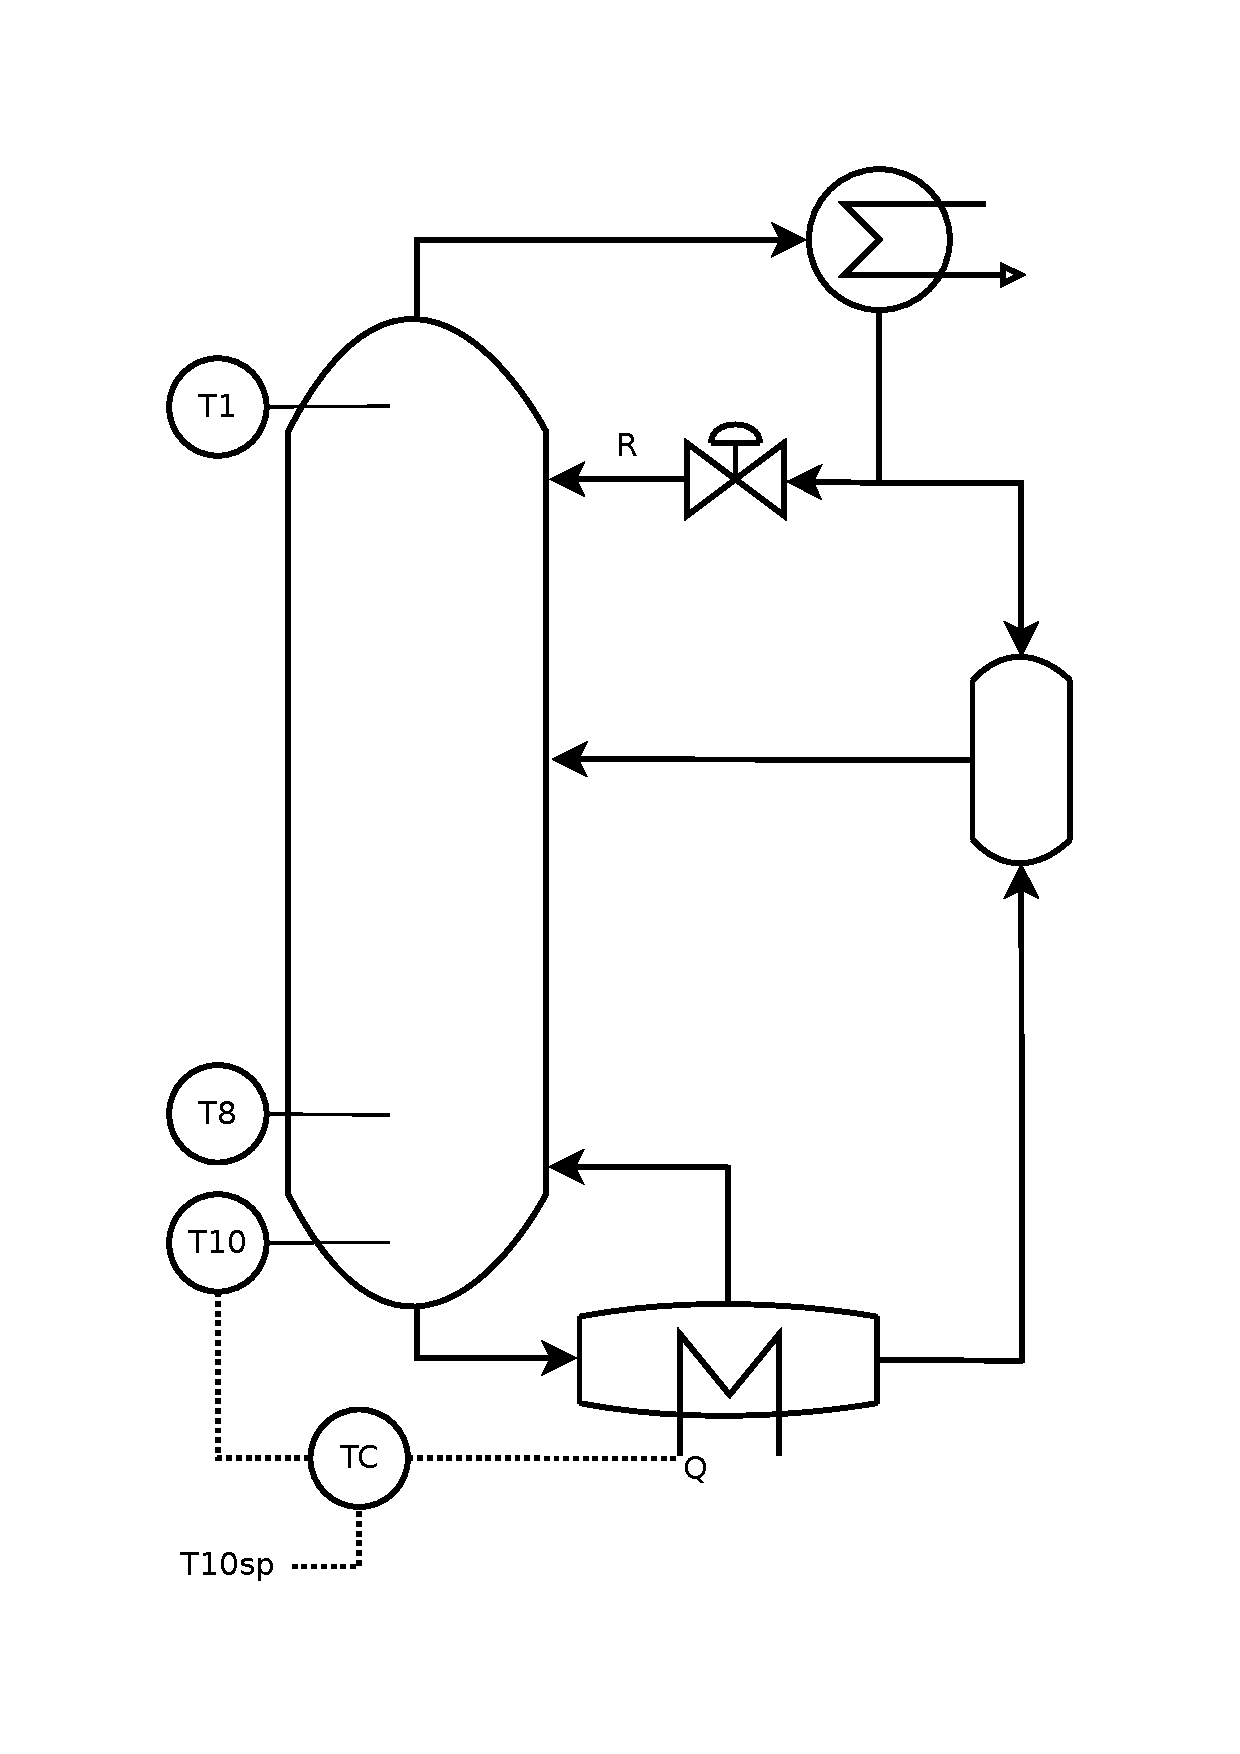
\includegraphics[width=8cm]{columnpfd.pdf}
    \beginpgfgraphicnamed{figure1}
    \scalebox{1}{% Graphic for TeX using PGF
% Title: /home/andre/GIT Repos/AHCampher_thesis/diagrams/columnpfd.dia
% Creator: Dia v0.97.1
% CreationDate: Thu Jan  6 17:23:45 2011
% For: andre
% \usepackage{tikz}
% The following commands are not supported in PSTricks at present
% We define them conditionally, so when they are implemented,
% this pgf file will use them.
\ifx\du\undefined
  \newlength{\du}
\fi
\setlength{\du}{15\unitlength}
\begin{tikzpicture}
\pgftransformxscale{0.803962}
\pgftransformyscale{-0.803962}
\definecolor{dialinecolor}{rgb}{0.000000, 0.000000, 0.000000}
\pgfsetstrokecolor{dialinecolor}
\definecolor{dialinecolor}{rgb}{1.000000, 1.000000, 1.000000}
\pgfsetfillcolor{dialinecolor}
\pgfsetlinewidth{0.100000\du}
\pgfsetdash{}{0pt}
\pgfsetdash{}{0pt}
\pgfsetbuttcap
\pgfsetmiterjoin
\pgfsetlinewidth{0.100000\du}
\pgfsetbuttcap
\pgfsetmiterjoin
\pgfsetdash{}{0pt}
\definecolor{dialinecolor}{rgb}{1.000000, 1.000000, 1.000000}
\pgfsetfillcolor{dialinecolor}
\fill (15.400000\du,11.560000\du)--(20.700000\du,11.560000\du)--(20.700000\du,25.240000\du)--(15.400000\du,25.240000\du)--cycle;
\pgfsetbuttcap
\pgfsetmiterjoin
\pgfsetdash{}{0pt}
\definecolor{dialinecolor}{rgb}{1.000000, 1.000000, 1.000000}
\pgfsetfillcolor{dialinecolor}
\pgfpathmoveto{\pgfpoint{15.400000\du}{11.560000\du}}
\pgfpathcurveto{\pgfpoint{18.050000\du}{7.000000\du}}{\pgfpoint{20.700000\du}{11.560000\du}}{\pgfpoint{20.700000\du}{11.560000\du}}
\pgfpathlineto{\pgfpoint{15.400000\du}{11.560000\du}}
\pgfusepath{fill}
\pgfsetbuttcap
\pgfsetmiterjoin
\pgfsetdash{}{0pt}
\definecolor{dialinecolor}{rgb}{1.000000, 1.000000, 1.000000}
\pgfsetfillcolor{dialinecolor}
\pgfpathmoveto{\pgfpoint{15.400000\du}{25.240000\du}}
\pgfpathcurveto{\pgfpoint{18.050000\du}{29.800000\du}}{\pgfpoint{20.700000\du}{25.240000\du}}{\pgfpoint{20.700000\du}{25.240000\du}}
\pgfpathlineto{\pgfpoint{15.400000\du}{25.240000\du}}
\pgfusepath{fill}
\pgfsetbuttcap
\pgfsetmiterjoin
\pgfsetdash{}{0pt}
\definecolor{dialinecolor}{rgb}{0.000000, 0.000000, 0.000000}
\pgfsetstrokecolor{dialinecolor}
\draw (15.400000\du,11.560000\du)--(15.400000\du,25.240000\du);
\pgfsetbuttcap
\pgfsetmiterjoin
\pgfsetdash{}{0pt}
\definecolor{dialinecolor}{rgb}{0.000000, 0.000000, 0.000000}
\pgfsetstrokecolor{dialinecolor}
\draw (20.700000\du,11.560000\du)--(20.700000\du,25.240000\du);
\pgfsetbuttcap
\pgfsetmiterjoin
\pgfsetdash{}{0pt}
\definecolor{dialinecolor}{rgb}{0.000000, 0.000000, 0.000000}
\pgfsetstrokecolor{dialinecolor}
\pgfpathmoveto{\pgfpoint{15.400000\du}{11.560000\du}}
\pgfpathcurveto{\pgfpoint{18.050000\du}{7.000000\du}}{\pgfpoint{20.700000\du}{11.560000\du}}{\pgfpoint{20.700000\du}{11.560000\du}}
\pgfusepath{stroke}
\pgfsetbuttcap
\pgfsetmiterjoin
\pgfsetdash{}{0pt}
\definecolor{dialinecolor}{rgb}{0.000000, 0.000000, 0.000000}
\pgfsetstrokecolor{dialinecolor}
\pgfpathmoveto{\pgfpoint{15.400000\du}{25.240000\du}}
\pgfpathcurveto{\pgfpoint{18.050000\du}{29.800000\du}}{\pgfpoint{20.700000\du}{25.240000\du}}{\pgfpoint{20.700000\du}{25.240000\du}}
\pgfusepath{stroke}
\pgfsetlinewidth{0.100000\du}
\pgfsetdash{}{0pt}
\pgfsetdash{}{0pt}
\pgfsetbuttcap
\pgfsetmiterjoin
\pgfsetlinewidth{0.100000\du}
\pgfsetbuttcap
\pgfsetmiterjoin
\pgfsetdash{}{0pt}
\definecolor{dialinecolor}{rgb}{1.000000, 1.000000, 1.000000}
\pgfsetfillcolor{dialinecolor}
\pgfpathellipse{\pgfpoint{29.008333\du}{8.008333\du}}{\pgfpoint{1.445833\du}{0\du}}{\pgfpoint{0\du}{1.445833\du}}
\pgfusepath{fill}
\definecolor{dialinecolor}{rgb}{0.000000, 0.000000, 0.000000}
\pgfsetstrokecolor{dialinecolor}
\pgfpathellipse{\pgfpoint{29.008333\du}{8.008333\du}}{\pgfpoint{1.445833\du}{0\du}}{\pgfpoint{0\du}{1.445833\du}}
\pgfusepath{stroke}
\pgfsetbuttcap
\pgfsetmiterjoin
\pgfsetdash{}{0pt}
\definecolor{dialinecolor}{rgb}{0.000000, 0.000000, 0.000000}
\pgfsetstrokecolor{dialinecolor}
\draw (31.177083\du,7.285417\du)--(28.285417\du,7.285417\du)--(29.008333\du,8.008333\du)--(28.285417\du,8.731250\du)--(31.538542\du,8.731250\du);
\pgfsetbuttcap
\pgfsetmiterjoin
\pgfsetdash{}{0pt}
\definecolor{dialinecolor}{rgb}{1.000000, 1.000000, 1.000000}
\pgfsetfillcolor{dialinecolor}
\fill (31.538542\du,8.550521\du)--(31.900000\du,8.731250\du)--(31.538542\du,8.911979\du)--cycle;
\definecolor{dialinecolor}{rgb}{0.000000, 0.000000, 0.000000}
\pgfsetstrokecolor{dialinecolor}
\draw (31.538542\du,8.550521\du)--(31.900000\du,8.731250\du)--(31.538542\du,8.911979\du)--cycle;
\pgfsetlinewidth{0.100000\du}
\pgfsetdash{}{0pt}
\pgfsetdash{}{0pt}
\pgfsetbuttcap
\pgfsetmiterjoin
\pgfsetlinewidth{0.100000\du}
\pgfsetbuttcap
\pgfsetmiterjoin
\pgfsetdash{}{0pt}
\definecolor{dialinecolor}{rgb}{1.000000, 1.000000, 1.000000}
\pgfsetfillcolor{dialinecolor}
\pgfpathmoveto{\pgfpoint{23.868750\du}{12.504673\du}}
\pgfpathcurveto{\pgfpoint{23.868750\du}{12.000000\du}}{\pgfpoint{24.868750\du}{12.000000\du}}{\pgfpoint{24.868750\du}{12.504673\du}}
\pgfpathlineto{\pgfpoint{23.868750\du}{12.504673\du}}
\pgfusepath{fill}
\pgfsetbuttcap
\pgfsetmiterjoin
\pgfsetdash{}{0pt}
\definecolor{dialinecolor}{rgb}{1.000000, 1.000000, 1.000000}
\pgfsetfillcolor{dialinecolor}
\fill (23.368750\du,12.504673\du)--(25.368750\du,14.000000\du)--(25.368750\du,12.504673\du)--(23.368750\du,14.000000\du)--cycle;
\pgfsetbuttcap
\pgfsetmiterjoin
\pgfsetdash{}{0pt}
\definecolor{dialinecolor}{rgb}{0.000000, 0.000000, 0.000000}
\pgfsetstrokecolor{dialinecolor}
\draw (23.368750\du,12.504673\du)--(25.368750\du,14.000000\du)--(25.368750\du,12.504673\du)--(23.368750\du,14.000000\du)--cycle;
\pgfsetbuttcap
\pgfsetmiterjoin
\pgfsetdash{}{0pt}
\definecolor{dialinecolor}{rgb}{0.000000, 0.000000, 0.000000}
\pgfsetstrokecolor{dialinecolor}
\draw (24.368750\du,13.252336\du)--(24.368750\du,12.504673\du);
\pgfsetbuttcap
\pgfsetmiterjoin
\pgfsetdash{}{0pt}
\definecolor{dialinecolor}{rgb}{0.000000, 0.000000, 0.000000}
\pgfsetstrokecolor{dialinecolor}
\draw (23.868750\du,12.504673\du)--(24.868750\du,12.504673\du);
\pgfsetbuttcap
\pgfsetmiterjoin
\pgfsetdash{}{0pt}
\definecolor{dialinecolor}{rgb}{0.000000, 0.000000, 0.000000}
\pgfsetstrokecolor{dialinecolor}
\pgfpathmoveto{\pgfpoint{23.868750\du}{12.504673\du}}
\pgfpathcurveto{\pgfpoint{23.868750\du}{12.000000\du}}{\pgfpoint{24.868750\du}{12.000000\du}}{\pgfpoint{24.868750\du}{12.504673\du}}
\pgfusepath{stroke}
\pgfsetlinewidth{0.100000\du}
\pgfsetdash{}{0pt}
\pgfsetdash{}{0pt}
\pgfsetbuttcap
\pgfsetmiterjoin
\pgfsetlinewidth{0.100000\du}
\pgfsetbuttcap
\pgfsetmiterjoin
\pgfsetdash{}{0pt}
\definecolor{dialinecolor}{rgb}{1.000000, 1.000000, 1.000000}
\pgfsetfillcolor{dialinecolor}
\fill (28.000000\du,17.090000\du)--(30.000000\du,17.090000\du)--(30.000000\du,20.360000\du)--(28.000000\du,20.360000\du)--cycle;
\pgfsetbuttcap
\pgfsetmiterjoin
\pgfsetdash{}{0pt}
\definecolor{dialinecolor}{rgb}{1.000000, 1.000000, 1.000000}
\pgfsetfillcolor{dialinecolor}
\pgfpathmoveto{\pgfpoint{28.000000\du}{17.090000\du}}
\pgfpathcurveto{\pgfpoint{29.000000\du}{16.000000\du}}{\pgfpoint{30.000000\du}{17.090000\du}}{\pgfpoint{30.000000\du}{17.090000\du}}
\pgfpathlineto{\pgfpoint{28.000000\du}{17.090000\du}}
\pgfusepath{fill}
\pgfsetbuttcap
\pgfsetmiterjoin
\pgfsetdash{}{0pt}
\definecolor{dialinecolor}{rgb}{1.000000, 1.000000, 1.000000}
\pgfsetfillcolor{dialinecolor}
\pgfpathmoveto{\pgfpoint{28.000000\du}{20.360000\du}}
\pgfpathcurveto{\pgfpoint{29.000000\du}{21.450000\du}}{\pgfpoint{30.000000\du}{20.360000\du}}{\pgfpoint{30.000000\du}{20.360000\du}}
\pgfpathlineto{\pgfpoint{28.000000\du}{20.360000\du}}
\pgfusepath{fill}
\pgfsetbuttcap
\pgfsetmiterjoin
\pgfsetdash{}{0pt}
\definecolor{dialinecolor}{rgb}{0.000000, 0.000000, 0.000000}
\pgfsetstrokecolor{dialinecolor}
\draw (28.000000\du,17.090000\du)--(28.000000\du,20.360000\du);
\pgfsetbuttcap
\pgfsetmiterjoin
\pgfsetdash{}{0pt}
\definecolor{dialinecolor}{rgb}{0.000000, 0.000000, 0.000000}
\pgfsetstrokecolor{dialinecolor}
\draw (30.000000\du,17.090000\du)--(30.000000\du,20.360000\du);
\pgfsetbuttcap
\pgfsetmiterjoin
\pgfsetdash{}{0pt}
\definecolor{dialinecolor}{rgb}{0.000000, 0.000000, 0.000000}
\pgfsetstrokecolor{dialinecolor}
\pgfpathmoveto{\pgfpoint{28.000000\du}{17.090000\du}}
\pgfpathcurveto{\pgfpoint{29.000000\du}{16.000000\du}}{\pgfpoint{30.000000\du}{17.090000\du}}{\pgfpoint{30.000000\du}{17.090000\du}}
\pgfusepath{stroke}
\pgfsetbuttcap
\pgfsetmiterjoin
\pgfsetdash{}{0pt}
\definecolor{dialinecolor}{rgb}{0.000000, 0.000000, 0.000000}
\pgfsetstrokecolor{dialinecolor}
\pgfpathmoveto{\pgfpoint{28.000000\du}{20.360000\du}}
\pgfpathcurveto{\pgfpoint{29.000000\du}{21.450000\du}}{\pgfpoint{30.000000\du}{20.360000\du}}{\pgfpoint{30.000000\du}{20.360000\du}}
\pgfusepath{stroke}
\pgfsetlinewidth{0.100000\du}
\pgfsetdash{}{0pt}
\pgfsetdash{}{0pt}
\pgfsetbuttcap
{
\definecolor{dialinecolor}{rgb}{0.000000, 0.000000, 0.000000}
\pgfsetfillcolor{dialinecolor}
% was here!!!
\pgfsetarrowsend{stealth}
\definecolor{dialinecolor}{rgb}{0.000000, 0.000000, 0.000000}
\pgfsetstrokecolor{dialinecolor}
\draw (28.000000\du,19.000000\du)--(20.800000\du,19.000000\du);
}
\pgfsetlinewidth{0.100000\du}
\pgfsetdash{}{0pt}
\pgfsetdash{}{0pt}
\pgfsetbuttcap
\pgfsetmiterjoin
\pgfsetlinewidth{0.100000\du}
\pgfsetbuttcap
\pgfsetmiterjoin
\pgfsetdash{}{0pt}
\definecolor{dialinecolor}{rgb}{1.000000, 1.000000, 1.000000}
\pgfsetfillcolor{dialinecolor}
\fill (21.382800\du,27.114200\du)--(27.482800\du,27.114200\du)--(27.482800\du,28.884200\du)--(21.382800\du,28.884200\du)--cycle;
\pgfsetbuttcap
\pgfsetmiterjoin
\pgfsetdash{}{0pt}
\definecolor{dialinecolor}{rgb}{1.000000, 1.000000, 1.000000}
\pgfsetfillcolor{dialinecolor}
\pgfpathmoveto{\pgfpoint{21.382800\du}{27.114200\du}}
\pgfpathcurveto{\pgfpoint{24.432800\du}{26.524200\du}}{\pgfpoint{27.482800\du}{27.114200\du}}{\pgfpoint{27.482800\du}{27.114200\du}}
\pgfpathlineto{\pgfpoint{21.382800\du}{27.114200\du}}
\pgfusepath{fill}
\pgfsetbuttcap
\pgfsetmiterjoin
\pgfsetdash{}{0pt}
\definecolor{dialinecolor}{rgb}{1.000000, 1.000000, 1.000000}
\pgfsetfillcolor{dialinecolor}
\pgfpathmoveto{\pgfpoint{21.382800\du}{28.884200\du}}
\pgfpathcurveto{\pgfpoint{24.432800\du}{29.474200\du}}{\pgfpoint{27.482800\du}{28.884200\du}}{\pgfpoint{27.482800\du}{28.884200\du}}
\pgfpathlineto{\pgfpoint{21.382800\du}{28.884200\du}}
\pgfusepath{fill}
\pgfsetbuttcap
\pgfsetmiterjoin
\pgfsetdash{}{0pt}
\definecolor{dialinecolor}{rgb}{0.000000, 0.000000, 0.000000}
\pgfsetstrokecolor{dialinecolor}
\draw (21.382800\du,27.114200\du)--(21.382800\du,28.884200\du);
\pgfsetbuttcap
\pgfsetmiterjoin
\pgfsetdash{}{0pt}
\definecolor{dialinecolor}{rgb}{0.000000, 0.000000, 0.000000}
\pgfsetstrokecolor{dialinecolor}
\draw (27.482800\du,27.114200\du)--(27.482800\du,28.884200\du);
\pgfsetbuttcap
\pgfsetmiterjoin
\pgfsetdash{}{0pt}
\definecolor{dialinecolor}{rgb}{0.000000, 0.000000, 0.000000}
\pgfsetstrokecolor{dialinecolor}
\pgfpathmoveto{\pgfpoint{21.382800\du}{27.114200\du}}
\pgfpathcurveto{\pgfpoint{24.432800\du}{26.524200\du}}{\pgfpoint{27.482800\du}{27.114200\du}}{\pgfpoint{27.482800\du}{27.114200\du}}
\pgfusepath{stroke}
\pgfsetbuttcap
\pgfsetmiterjoin
\pgfsetdash{}{0pt}
\definecolor{dialinecolor}{rgb}{0.000000, 0.000000, 0.000000}
\pgfsetstrokecolor{dialinecolor}
\pgfpathmoveto{\pgfpoint{21.382800\du}{28.884200\du}}
\pgfpathcurveto{\pgfpoint{24.432800\du}{29.474200\du}}{\pgfpoint{27.482800\du}{28.884200\du}}{\pgfpoint{27.482800\du}{28.884200\du}}
\pgfusepath{stroke}
\pgfsetlinewidth{0.100000\du}
\pgfsetdash{}{0pt}
\pgfsetdash{}{0pt}
\pgfsetbuttcap
\pgfsetmiterjoin
\pgfsetlinewidth{0.100000\du}
\pgfsetbuttcap
\pgfsetmiterjoin
\pgfsetdash{}{0pt}
\definecolor{dialinecolor}{rgb}{0.000000, 0.000000, 0.000000}
\pgfsetstrokecolor{dialinecolor}
\draw (23.439100\du,29.967925\du)--(23.439100\du,27.464800\du)--(24.460975\du,28.716363\du)--(25.482850\du,27.464800\du)--(25.482850\du,29.967925\du);
\pgfsetlinewidth{0.100000\du}
\pgfsetdash{}{0pt}
\pgfsetdash{}{0pt}
\pgfsetbuttcap
{
\definecolor{dialinecolor}{rgb}{0.000000, 0.000000, 0.000000}
\pgfsetfillcolor{dialinecolor}
% was here!!!
\definecolor{dialinecolor}{rgb}{0.000000, 0.000000, 0.000000}
\pgfsetstrokecolor{dialinecolor}
\draw (24.432800\du,26.848700\du)--(24.427000\du,24.002300\du);
}
\pgfsetlinewidth{0.100000\du}
\pgfsetdash{}{0pt}
\pgfsetdash{}{0pt}
\pgfsetbuttcap
{
\definecolor{dialinecolor}{rgb}{0.000000, 0.000000, 0.000000}
\pgfsetfillcolor{dialinecolor}
% was here!!!
\pgfsetarrowsend{stealth}
\definecolor{dialinecolor}{rgb}{0.000000, 0.000000, 0.000000}
\pgfsetstrokecolor{dialinecolor}
\draw (24.427000\du,24.039800\du)--(20.752000\du,24.039800\du);
}
\pgfsetlinewidth{0.100000\du}
\pgfsetdash{}{0pt}
\pgfsetdash{}{0pt}
\pgfsetbuttcap
{
\definecolor{dialinecolor}{rgb}{0.000000, 0.000000, 0.000000}
\pgfsetfillcolor{dialinecolor}
% was here!!!
\definecolor{dialinecolor}{rgb}{0.000000, 0.000000, 0.000000}
\pgfsetstrokecolor{dialinecolor}
\draw (27.482800\du,27.999200\du)--(29.000000\du,28.000000\du);
}
\pgfsetlinewidth{0.100000\du}
\pgfsetdash{}{0pt}
\pgfsetdash{}{0pt}
\pgfsetbuttcap
{
\definecolor{dialinecolor}{rgb}{0.000000, 0.000000, 0.000000}
\pgfsetfillcolor{dialinecolor}
% was here!!!
\pgfsetarrowsend{stealth}
\definecolor{dialinecolor}{rgb}{0.000000, 0.000000, 0.000000}
\pgfsetstrokecolor{dialinecolor}
\draw (29.000000\du,28.000000\du)--(29.000000\du,20.850500\du);
}
\pgfsetlinewidth{0.100000\du}
\pgfsetdash{}{0pt}
\pgfsetdash{}{0pt}
\pgfsetbuttcap
\pgfsetmiterjoin
\pgfsetlinewidth{0.100000\du}
\pgfsetbuttcap
\pgfsetmiterjoin
\pgfsetdash{}{0pt}
\definecolor{dialinecolor}{rgb}{1.000000, 1.000000, 1.000000}
\pgfsetfillcolor{dialinecolor}
\pgfpathellipse{\pgfpoint{14.000000\du}{12.000000\du}}{\pgfpoint{1.000000\du}{0\du}}{\pgfpoint{0\du}{1.000000\du}}
\pgfusepath{fill}
\definecolor{dialinecolor}{rgb}{0.000000, 0.000000, 0.000000}
\pgfsetstrokecolor{dialinecolor}
\pgfpathellipse{\pgfpoint{14.000000\du}{12.000000\du}}{\pgfpoint{1.000000\du}{0\du}}{\pgfpoint{0\du}{1.000000\du}}
\pgfusepath{stroke}
% setfont left to latex
\definecolor{dialinecolor}{rgb}{0.000000, 0.000000, 0.000000}
\pgfsetstrokecolor{dialinecolor}
\node at (14.000000\du,12.000000\du){$T_1$};
\pgfsetlinewidth{0.100000\du}
\pgfsetdash{}{0pt}
\pgfsetdash{}{0pt}
\pgfsetbuttcap
\pgfsetmiterjoin
\pgfsetlinewidth{0.100000\du}
\pgfsetbuttcap
\pgfsetmiterjoin
\pgfsetdash{}{0pt}
\definecolor{dialinecolor}{rgb}{1.000000, 1.000000, 1.000000}
\pgfsetfillcolor{dialinecolor}
\pgfpathellipse{\pgfpoint{13.961900\du}{25.600600\du}}{\pgfpoint{1.000000\du}{0\du}}{\pgfpoint{0\du}{1.000000\du}}
\pgfusepath{fill}
\definecolor{dialinecolor}{rgb}{0.000000, 0.000000, 0.000000}
\pgfsetstrokecolor{dialinecolor}
\pgfpathellipse{\pgfpoint{13.961900\du}{25.600600\du}}{\pgfpoint{1.000000\du}{0\du}}{\pgfpoint{0\du}{1.000000\du}}
\pgfusepath{stroke}
% setfont left to latex
\definecolor{dialinecolor}{rgb}{0.000000, 0.000000, 0.000000}
\pgfsetstrokecolor{dialinecolor}
\node at (13.961900\du,25.600600\du){$T_{10}$};
\pgfsetlinewidth{0.050000\du}
\pgfsetdash{}{0pt}
\pgfsetdash{}{0pt}
\pgfsetbuttcap
{
\definecolor{dialinecolor}{rgb}{0.000000, 0.000000, 0.000000}
\pgfsetfillcolor{dialinecolor}
% was here!!!
\definecolor{dialinecolor}{rgb}{0.000000, 0.000000, 0.000000}
\pgfsetstrokecolor{dialinecolor}
\draw (15.000000\du,12.000000\du)--(17.516200\du,11.980470\du);
}
\pgfsetlinewidth{0.050000\du}
\pgfsetdash{}{0pt}
\pgfsetdash{}{0pt}
\pgfsetbuttcap
{
\definecolor{dialinecolor}{rgb}{0.000000, 0.000000, 0.000000}
\pgfsetfillcolor{dialinecolor}
% was here!!!
\definecolor{dialinecolor}{rgb}{0.000000, 0.000000, 0.000000}
\pgfsetstrokecolor{dialinecolor}
\draw (14.961900\du,25.600600\du)--(17.493300\du,25.590700\du);
}
\pgfsetlinewidth{0.100000\du}
\pgfsetdash{}{0pt}
\pgfsetdash{}{0pt}
\pgfsetbuttcap
\pgfsetmiterjoin
\pgfsetlinewidth{0.100000\du}
\pgfsetbuttcap
\pgfsetmiterjoin
\pgfsetdash{}{0pt}
\definecolor{dialinecolor}{rgb}{1.000000, 1.000000, 1.000000}
\pgfsetfillcolor{dialinecolor}
\pgfpathellipse{\pgfpoint{16.861900\du}{30.018000\du}}{\pgfpoint{1.000000\du}{0\du}}{\pgfpoint{0\du}{1.000000\du}}
\pgfusepath{fill}
\definecolor{dialinecolor}{rgb}{0.000000, 0.000000, 0.000000}
\pgfsetstrokecolor{dialinecolor}
\pgfpathellipse{\pgfpoint{16.861900\du}{30.018000\du}}{\pgfpoint{1.000000\du}{0\du}}{\pgfpoint{0\du}{1.000000\du}}
\pgfusepath{stroke}
% setfont left to latex
\definecolor{dialinecolor}{rgb}{0.000000, 0.000000, 0.000000}
\pgfsetstrokecolor{dialinecolor}
\node at (16.861900\du,30.018000\du){TC};
\pgfsetlinewidth{0.100000\du}
\pgfsetdash{{\pgflinewidth}{0.200000\du}}{0cm}
\pgfsetdash{{\pgflinewidth}{0.200000\du}}{0cm}
\pgfsetmiterjoin
\pgfsetbuttcap
{
\definecolor{dialinecolor}{rgb}{0.000000, 0.000000, 0.000000}
\pgfsetfillcolor{dialinecolor}
% was here!!!
{\pgfsetcornersarced{\pgfpoint{0.000000\du}{0.000000\du}}\definecolor{dialinecolor}{rgb}{0.000000, 0.000000, 0.000000}
\pgfsetstrokecolor{dialinecolor}
\draw (13.961900\du,26.600600\du)--(13.961900\du,30.018000\du)--(15.861900\du,30.018000\du);
}}
\pgfsetlinewidth{0.100000\du}
\pgfsetdash{{\pgflinewidth}{0.200000\du}}{0cm}
\pgfsetdash{{\pgflinewidth}{0.200000\du}}{0cm}
\pgfsetmiterjoin
\pgfsetbuttcap
{
\definecolor{dialinecolor}{rgb}{0.000000, 0.000000, 0.000000}
\pgfsetfillcolor{dialinecolor}
% was here!!!
{\pgfsetcornersarced{\pgfpoint{0.000000\du}{0.000000\du}}\definecolor{dialinecolor}{rgb}{0.000000, 0.000000, 0.000000}
\pgfsetstrokecolor{dialinecolor}
\draw (17.861900\du,30.018000\du)--(20.611900\du,30.018000\du)--(20.611900\du,30.021100\du)--(23.361900\du,30.021100\du);
}}
% setfont left to latex
\definecolor{dialinecolor}{rgb}{0.000000, 0.000000, 0.000000}
\pgfsetstrokecolor{dialinecolor}
\node[anchor=west] at (13.186900\du,32.412500\du){$T_{10~sp}$};
\pgfsetlinewidth{0.100000\du}
\pgfsetdash{{\pgflinewidth}{0.200000\du}}{0cm}
\pgfsetdash{{\pgflinewidth}{0.200000\du}}{0cm}
\pgfsetmiterjoin
\pgfsetbuttcap
{
\definecolor{dialinecolor}{rgb}{0.000000, 0.000000, 0.000000}
\pgfsetfillcolor{dialinecolor}
% was here!!!
{\pgfsetcornersarced{\pgfpoint{0.000000\du}{0.000000\du}}\definecolor{dialinecolor}{rgb}{0.000000, 0.000000, 0.000000}
\pgfsetstrokecolor{dialinecolor}
\draw (15.486900\du,32.237500\du)--(16.861900\du,32.237500\du)--(16.861900\du,31.018000\du);
}}
% setfont left to latex
\definecolor{dialinecolor}{rgb}{0.000000, 0.000000, 0.000000}
\pgfsetstrokecolor{dialinecolor}
\node[anchor=west] at (23.511900\du,30.437500\du){$Q$};
% setfont left to latex
\definecolor{dialinecolor}{rgb}{0.000000, 0.000000, 0.000000}
\pgfsetstrokecolor{dialinecolor}
\node[anchor=west] at (21.500000\du,12.500000\du){$R$};
\pgfsetlinewidth{0.100000\du}
\pgfsetdash{}{0pt}
\pgfsetdash{}{0pt}
\pgfsetbuttcap
\pgfsetmiterjoin
\pgfsetlinewidth{0.100000\du}
\pgfsetbuttcap
\pgfsetmiterjoin
\pgfsetdash{}{0pt}
\definecolor{dialinecolor}{rgb}{1.000000, 1.000000, 1.000000}
\pgfsetfillcolor{dialinecolor}
\pgfpathellipse{\pgfpoint{14.000000\du}{23.000000\du}}{\pgfpoint{1.000000\du}{0\du}}{\pgfpoint{0\du}{1.000000\du}}
\pgfusepath{fill}
\definecolor{dialinecolor}{rgb}{0.000000, 0.000000, 0.000000}
\pgfsetstrokecolor{dialinecolor}
\pgfpathellipse{\pgfpoint{14.000000\du}{23.000000\du}}{\pgfpoint{1.000000\du}{0\du}}{\pgfpoint{0\du}{1.000000\du}}
\pgfusepath{stroke}
% setfont left to latex
\definecolor{dialinecolor}{rgb}{0.000000, 0.000000, 0.000000}
\pgfsetstrokecolor{dialinecolor}
\node at (14.000000\du,23.000000\du){$T_8$};
\pgfsetlinewidth{0.050000\du}
\pgfsetdash{}{0pt}
\pgfsetdash{}{0pt}
\pgfsetbuttcap
{
\definecolor{dialinecolor}{rgb}{0.000000, 0.000000, 0.000000}
\pgfsetfillcolor{dialinecolor}
% was here!!!
\definecolor{dialinecolor}{rgb}{0.000000, 0.000000, 0.000000}
\pgfsetstrokecolor{dialinecolor}
\draw (15.000000\du,23.000000\du)--(17.516200\du,22.980470\du);
}
\pgfsetlinewidth{0.100000\du}
\pgfsetdash{}{0pt}
\pgfsetdash{}{0pt}
\pgfsetbuttcap
{
\definecolor{dialinecolor}{rgb}{0.000000, 0.000000, 0.000000}
\pgfsetfillcolor{dialinecolor}
% was here!!!
\definecolor{dialinecolor}{rgb}{0.000000, 0.000000, 0.000000}
\pgfsetstrokecolor{dialinecolor}
\draw (29.000000\du,9.500000\du)--(29.000000\du,13.400000\du);
}
\pgfsetlinewidth{0.100000\du}
\pgfsetdash{}{0pt}
\pgfsetdash{}{0pt}
\pgfsetbuttcap
{
\definecolor{dialinecolor}{rgb}{0.000000, 0.000000, 0.000000}
\pgfsetfillcolor{dialinecolor}
% was here!!!
\pgfsetarrowsend{stealth}
\definecolor{dialinecolor}{rgb}{0.000000, 0.000000, 0.000000}
\pgfsetstrokecolor{dialinecolor}
\draw (23.331250\du,13.268750\du)--(20.731250\du,13.268750\du);
}
\pgfsetlinewidth{0.100000\du}
\pgfsetdash{}{0pt}
\pgfsetdash{}{0pt}
\pgfsetbuttcap
{
\definecolor{dialinecolor}{rgb}{0.000000, 0.000000, 0.000000}
\pgfsetfillcolor{dialinecolor}
% was here!!!
\pgfsetarrowsend{stealth}
\definecolor{dialinecolor}{rgb}{0.000000, 0.000000, 0.000000}
\pgfsetstrokecolor{dialinecolor}
\draw (18.000000\du,8.000000\du)--(27.500000\du,8.000000\du);
}
\pgfsetlinewidth{0.100000\du}
\pgfsetdash{}{0pt}
\pgfsetdash{}{0pt}
\pgfsetbuttcap
{
\definecolor{dialinecolor}{rgb}{0.000000, 0.000000, 0.000000}
\pgfsetfillcolor{dialinecolor}
% was here!!!
\pgfsetarrowsend{stealth}
\definecolor{dialinecolor}{rgb}{0.000000, 0.000000, 0.000000}
\pgfsetstrokecolor{dialinecolor}
\draw (18.000000\du,28.000000\du)--(21.382800\du,27.999200\du);
}
\pgfsetlinewidth{0.100000\du}
\pgfsetdash{}{0pt}
\pgfsetdash{}{0pt}
\pgfsetbuttcap
{
\definecolor{dialinecolor}{rgb}{0.000000, 0.000000, 0.000000}
\pgfsetfillcolor{dialinecolor}
% was here!!!
\pgfsetarrowsend{stealth}
\definecolor{dialinecolor}{rgb}{0.000000, 0.000000, 0.000000}
\pgfsetstrokecolor{dialinecolor}
\draw (29.000000\du,13.400000\du)--(29.000000\du,16.599500\du);
}
\pgfsetlinewidth{0.100000\du}
\pgfsetdash{}{0pt}
\pgfsetdash{}{0pt}
\pgfsetbuttcap
{
\definecolor{dialinecolor}{rgb}{0.000000, 0.000000, 0.000000}
\pgfsetfillcolor{dialinecolor}
% was here!!!
\pgfsetarrowsend{stealth}
\definecolor{dialinecolor}{rgb}{0.000000, 0.000000, 0.000000}
\pgfsetstrokecolor{dialinecolor}
\draw (28.993750\du,13.256250\du)--(25.393750\du,13.256250\du);
}
\pgfsetlinewidth{0.100000\du}
\pgfsetdash{}{0pt}
\pgfsetdash{}{0pt}
\pgfsetbuttcap
{
\definecolor{dialinecolor}{rgb}{0.000000, 0.000000, 0.000000}
\pgfsetfillcolor{dialinecolor}
% was here!!!
\definecolor{dialinecolor}{rgb}{0.000000, 0.000000, 0.000000}
\pgfsetstrokecolor{dialinecolor}
\draw (18.050625\du,7.960000\du)--(18.050625\du,9.500000\du);
}
\pgfsetlinewidth{0.100000\du}
\pgfsetdash{}{0pt}
\pgfsetdash{}{0pt}
\pgfsetbuttcap
{
\definecolor{dialinecolor}{rgb}{0.000000, 0.000000, 0.000000}
\pgfsetfillcolor{dialinecolor}
% was here!!!
\definecolor{dialinecolor}{rgb}{0.000000, 0.000000, 0.000000}
\pgfsetstrokecolor{dialinecolor}
\draw (18.050937\du,28.040000\du)--(18.050937\du,27.260000\du);
}
\end{tikzpicture}
}
    \endpgfgraphicnamed
  \caption[Laboratory distillation column photo and flow diagram]{Laboratory distillation column flow diagram.}
  \label{fig:columnpfd}
\end{figure}

The process model has been reduced to a $2\times2$ matrix.
Reflux flowrate ($R$, expressed as the milliamp signal to the control valve) and the setpoint of plate 10's temperature ($T_{10~sp}$) are the inputs, with the temperatures of plate 1 and 8 ($T_1\text{ and }T_{8}$) as the outputs.
The temperature controller between $T_{10~sp}$ and $Q$ is part of the column's baselayer controls and was added as a safety measure, should the advanced control layer fail.

Equation~\ref{eq:columnmodel} shows the steady-state gain model ($G$) of the column.
\begin{equation}
  \label{eq:columnmodel}
                 % R      T10sp
  G = \bpm -0.0575 & 0.96 \\       % T1
           -0.146  & 0.518 \\ \epm % T8
\end{equation}

Table~\ref{tab:columnopcon} lists the operating conditions of the distillation column.
The nominal operating point (in the output space) is; 68~\textcelsius\ ($T_1$) and 78~\textcelsius\ ($T_8$).
\begin{table}[htbp]
  \centering
  \begin{tabular}{llllll}
    \toprule
    \multicolumn{2}{c}{Variable} & \multicolumn{4}{c}{Constraints}\\
     && \multicolumn{2}{c}{Operating} & \multicolumn{2}{c}{Physical} \\
    \cmidrule(r){3-4} \cmidrule(r){5-6}
    && Low & High & Low & High \\ 
    \midrule
    Inputs &$R$ (mA)          & 11 & 15 & 4 & 20 \\
           &$T_{10~sp}$ (\textcelsius) & 78 & 82 & 25 & 90 \\[1.3ex]
    Outputs &$T_1$ (\textcelsius)     & 66 & 68 & 15 & 68 \\
            &$T_{8}$ (\textcelsius)   & 78 & 82 & 25 & 90 \\
    \bottomrule
  \end{tabular}
  \caption{Operating conditions of the laboratory distillation column.}
  \label{tab:columnopcon}
\end{table}

\subsection{Input and Output spaces}
From the data in table~\ref{tab:columnopcon} and equation~\ref{eq:columnmodel} the AIS and AOS of the laboratory distillation column can be generated as shown in figure~\ref{fig:columnaisaos}(a, b).
Take note that the operating limits for $R$, and the physical limits for $T_{10~sp}$ are used to construct the AIS.
The DOS, as described by the operating range of the outputs, is also shown in figure~\ref{fig:columnaisaos}(b, c).

\begin{figure}[htbp]
  \centering
    %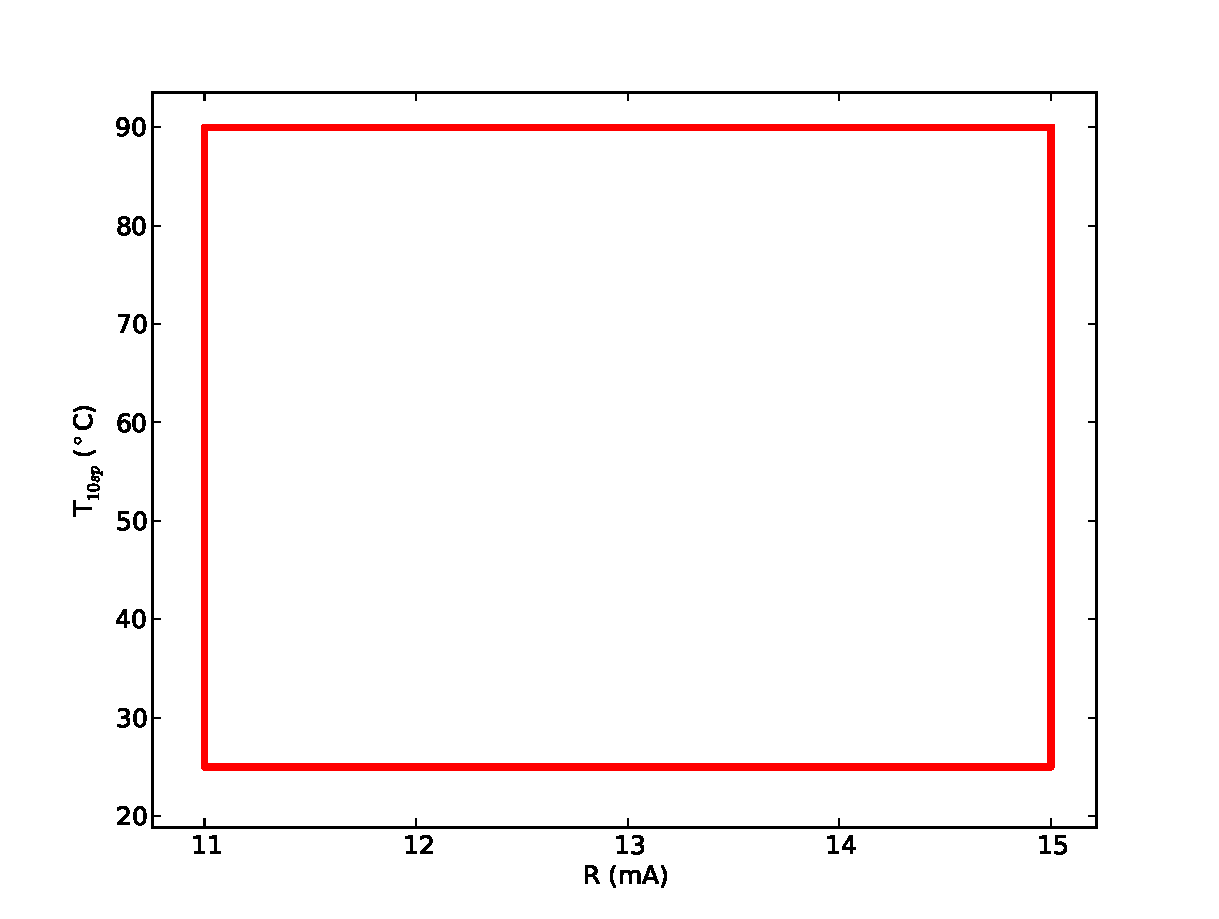
\includegraphics[width=8cm]{columnais.pdf}
    %\qquad
    %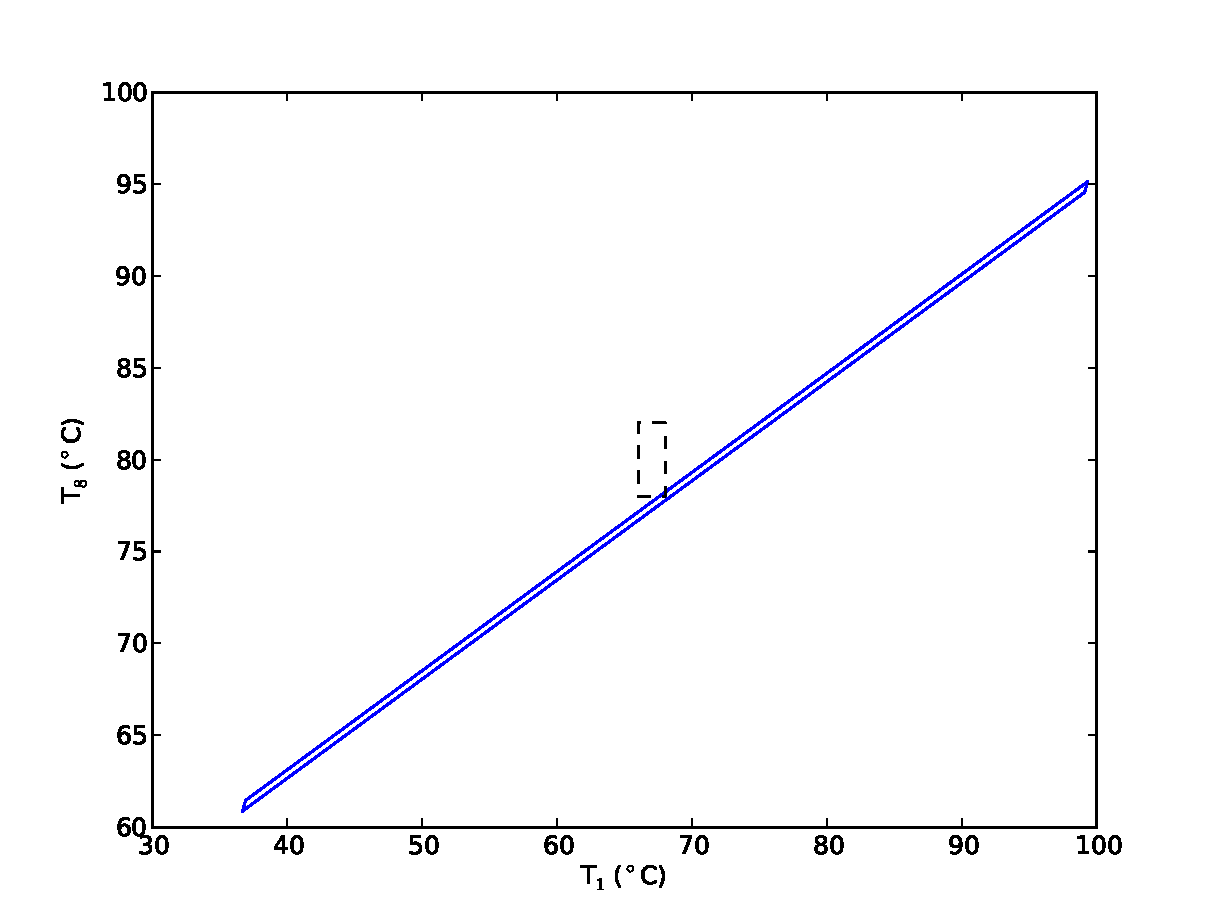
\includegraphics[width=8cm]{columnaos.pdf}
    %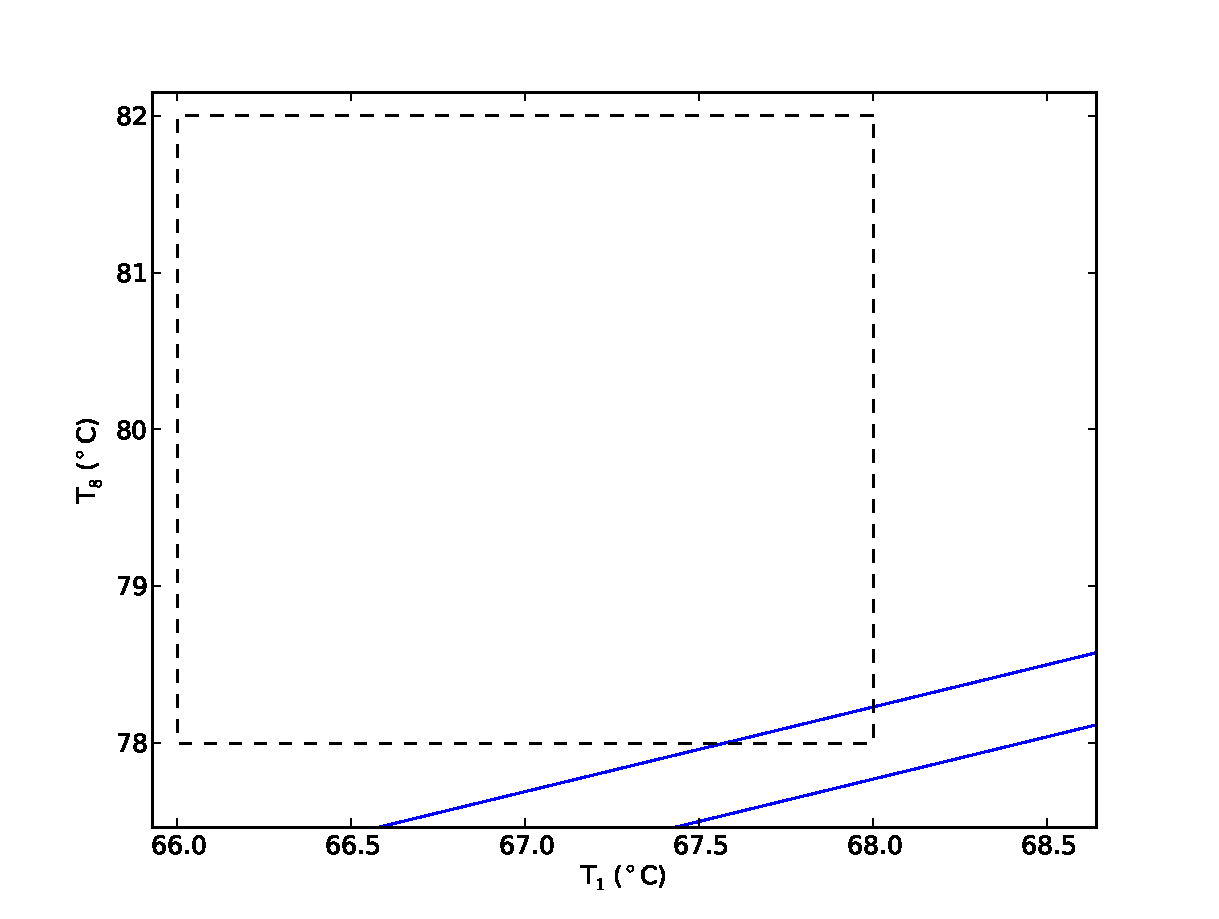
\includegraphics[width=8cm]{columnaosfocus.pdf}
    \beginpgfgraphicnamed{figure2a}
    \scalebox{1}{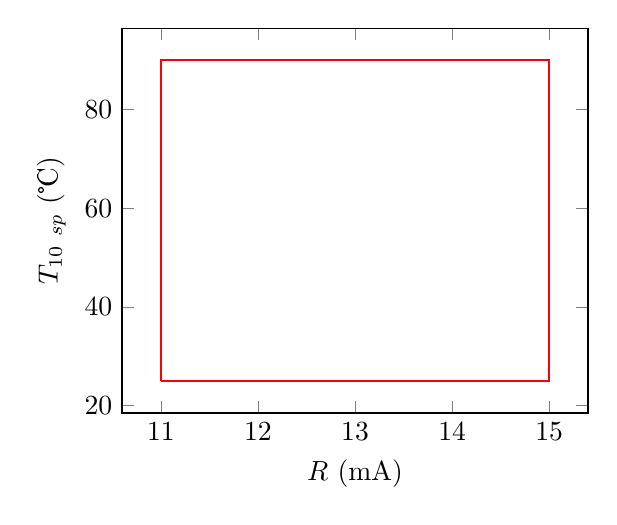
\begin{tikzpicture}
  \begin{axis}[
    width=7.5cm,
    xlabel=$R$~(mA),
    ylabel=$T_{10~sp}$~(\textcelsius)]
    \addplot[color=red,thick] coordinates {
      (11,25)
      (11,90)
      (15,90)
      (15,25)
      (11,25)
    };
  \end{axis}
\end{tikzpicture}
}
    \endpgfgraphicnamed
    \beginpgfgraphicnamed{figure2b}
    \scalebox{1}{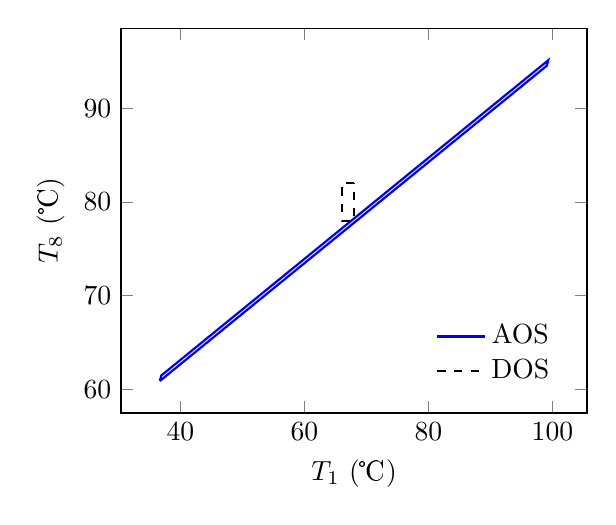
\begin{tikzpicture}
  \begin{axis}[
    width=7.5cm,
    xlabel=$T_1$~(\textcelsius),
    ylabel=$T_8$~(\textcelsius),
    legend style={
      draw=none,
      at={(0.95,0.05)},
      anchor=south east}]

    %AOS
    \addplot[color=blue,thick] coordinates {
      (36.685,  60.873) 
      (36.915,  61.457) 
      (99.315,  95.127) 
      (99.085,  94.543) 
      (36.685,  60.873) 
    };
    %DOS
    \addplot[color=black,thick,dashed] coordinates {
      (68.,  82.)
      (66.,  82.)
      (66.,  78.)
      (68.,  78.)
      (68.,  82.)
    };
    \legend{AOS,DOS}
  \end{axis}
\end{tikzpicture}
}
    \endpgfgraphicnamed
    \beginpgfgraphicnamed{figure2c}
    \scalebox{1}{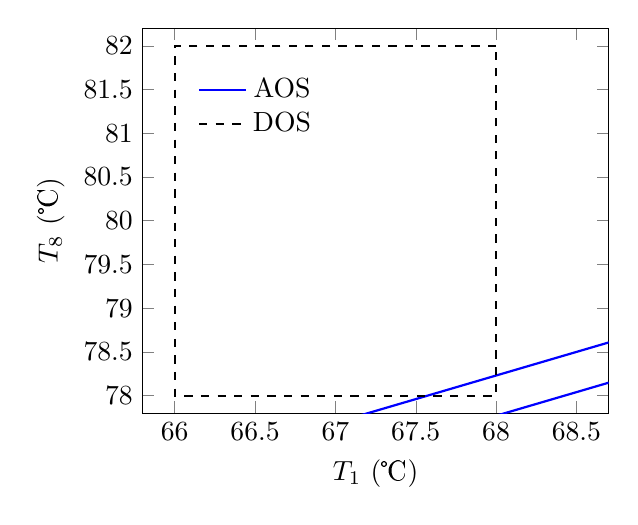
\begin{tikzpicture}
  \begin{axis}[
    width=7.5cm,
    xlabel=$T_1$~(\textcelsius),
    ylabel=$T_8$~(\textcelsius),
    xmin=65.8,xmax=68.7,ymin=77.8,ymax=82.2,
    xtick={66,66.5,...,68.5},
    ytick={78,78.5,...,82},
    legend style={
      draw=none,
      at={(0.10,0.90)},
      anchor=north west}]

    %AOS
    \addplot[color=blue,thick] coordinates {
      (36.685,  60.873) 
      (36.915,  61.457) 
      (99.315,  95.127) 
      (99.085,  94.543) 
      (36.685,  60.873) 
    };
    %DOS
    \addplot[color=black,thick,dashed] coordinates {
      (68.,  82.)
      (66.,  82.)
      (66.,  78.)
      (68.,  78.)
      (68.,  82.)
    };
    \legend{AOS,DOS}
  \end{axis}
\end{tikzpicture}
}
    \endpgfgraphicnamed
  \caption{AIS (a), AOS and DOS (b), and AOS$\cap$DOS (c) showing a very small operating region.}
  \label{fig:columnaisaos}
\end{figure}

Figure~\ref{fig:columnaisaos}(c) focuses on the intersection of the AOS and the DOS.
The calculated OI is 0.006 which confirms that only a very small operating region within the DOS is attainable.
It is also clear that the upper limit of 82~\textcelsius\ on $T_8$ is unrealistic as the maximum value of $T_8$ (in the desired operating region) is only 78.2~\textcelsius.

\subsubsection{Constraint reformatting}
The DOS and AOS intersection in figure~\ref{fig:columnaisaos}(b, c) represents the largest desirable operating region for the column.
This region is described by the following constraints:
\begin{align*}
  T_1 &\leq 68\text{~\textcelsius} \\
  T_8 &\geq 78\text{~\textcelsius} \\
  0.88T_8-0.47T_1&\leq 36.56\text{~\textcelsius}
\end{align*}

This set of constraints need to be reformatted to be compatible with commercial MPC packages, as they only accept high and low limits on variables.
An unmeasured variable is added to the process model to implement the diagonal constraint ($0.88T_8-0.47T_1\leq 36.56$~\textcelsius).
Defining the new output $y_1$ and augmenting the process model (equation~\ref{eq:columnmodel}) as per equation~\ref{eq:linconoutput} results in the new process model (equation~\ref{eq:columnnewmodel}) shown below. With the new process model defined thus, the diagonal constraint can be expressed as {$y_1~\leq~36.56$~\textcelsius}.
\begin{equation}
  \label{eq:columnnewmodel}
  G_{new}= \bpm -0.0575 & 0.96 \\       % T1
                  -0.146  & 0.518 \\      % T8
                   0.0956 & 1.30 \\ \epm  %y1
\end{equation}


\subsection{Constraint changes}
Instead of using the full DOS and AOS intersection, an upper and lower limit constraint set within the intersection could be used (as shown in figure~\ref{fig:columnfitbox}).
This smaller constraint set will have a clamping effect on the input constraints of the system.

\begin{figure}[htbp]
  \centering
    %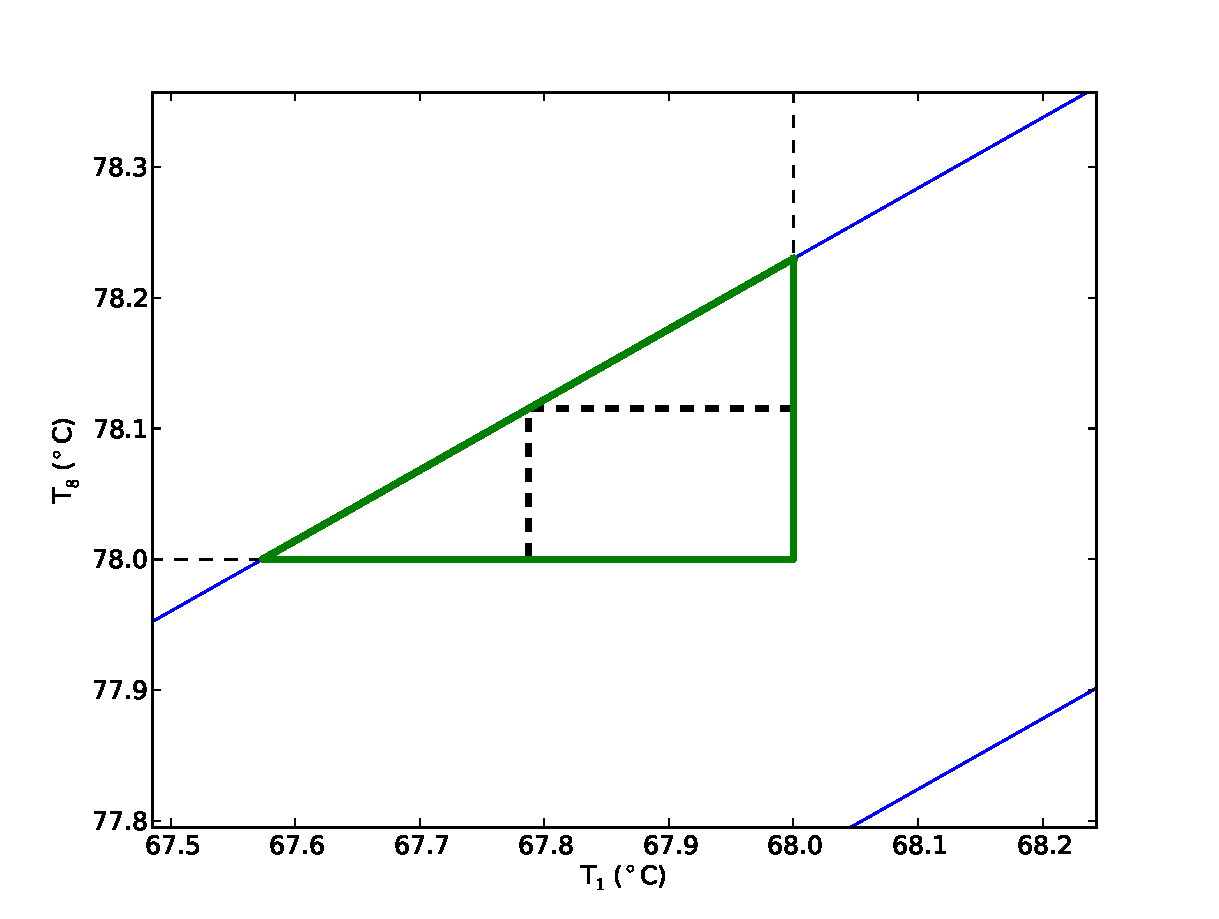
\includegraphics[width=8cm]{columnfitbox.pdf}
    \beginpgfgraphicnamed{figure3}
    \scalebox{1}{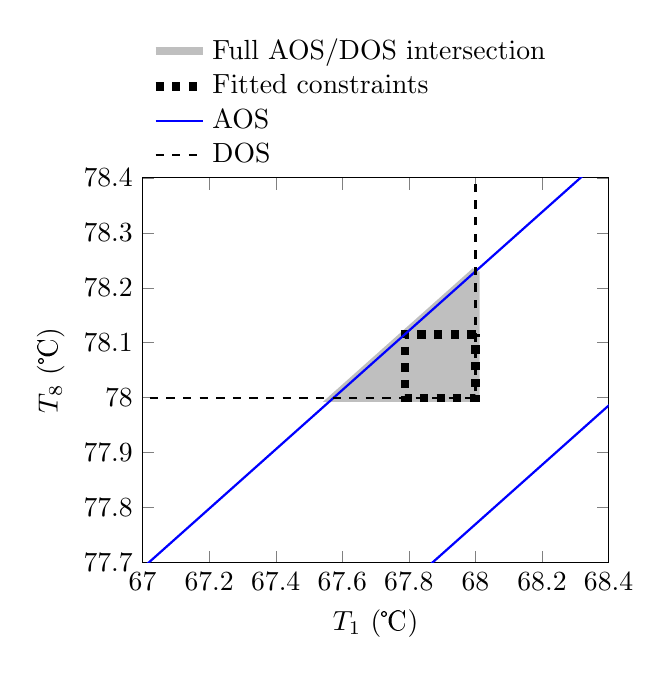
\begin{tikzpicture}
  \begin{axis}[
    width=7.5cm,
    xlabel=$T_1$~(\textcelsius),
    ylabel=$T_8$~(\textcelsius),
    xmin=67,xmax=68.4,ymin=77.7,ymax=78.4,
    xtick={67,67.2,...,68.4},
    ytick={77.7,77.8,...,78.4},
    legend style={
      draw=none,
      at={(0.0,1.0)},
      anchor=south west,
      cells={anchor=west}}]

    %intersection
    \addplot[fill=lightgray,color=lightgray,line width=3pt] coordinates {
      (68.      ,   78.2299483)
      (67.573841,   78.       )
      (68.      ,   78.       )
      (68.      ,   78.2299483)
    };
    %fitted cons
    \addplot[color=black,line width=3pt,dashed] coordinates {
      (67.99999975,  78.11504787)
      (67.78705642,  78.11504787)
      (67.78705642,  77.99999994)
      (67.99999975,  77.99999994)
      (67.99999975,  78.11504787)
    };
   %AOS
    \addplot[color=blue,thick] coordinates {
      (36.685,  60.873) 
      (36.915,  61.457) 
      (99.315,  95.127) 
      (99.085,  94.543) 
      (36.685,  60.873) 
    };
    %DOS
    \addplot[color=black,thick,dashed] coordinates {
      (68,  82)
      (66,  82)
      (66,  78)
      (68,  78)
      (68,  82)
    };
     \legend{Full AOS/DOS intersection,Fitted constraints,AOS,DOS}
  \end{axis}
\end{tikzpicture}
}
    \endpgfgraphicnamed
  \caption[Fitted constraints for the laboratory distillation column]{Intersection of AOS and DOS with fitted high and low limits for the column tray temperatures.}
  \label{fig:columnfitbox}
\end{figure}

The spaces shown in figure~\ref{fig:columnfitbox} are translated back to the input space as shown in figure~\ref{fig:columnconsinput}(a, b).
DISi represents the full AOS and DOS intersection in the input space, whereas DOSn represents the newly fitted high and low limits within the AOS and DOS intersection.
The effect of the constraint change is shown in figure~\ref{fig:columnconsinput}(b) as the transition from the shaded triangular constraint set to the parallelogram shaped dotted set.
From equation~\ref{eq:inputclamp} this corresponds to a 50\% clamping in the input space.

\begin{figure}[htbp]
  \centering
    \beginpgfgraphicnamed{figure4a}
    \scalebox{1}{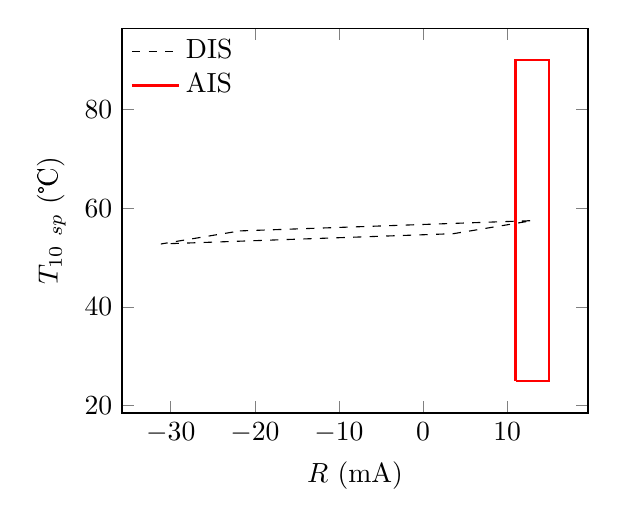
\begin{tikzpicture}
  \begin{axis}[
    width=7.5cm,
    xlabel=$R$~(mA),
    ylabel=$T_{10~sp}$~(\textcelsius),
    legend style={
      draw=none,
      at={(0.0,1.0)},
      anchor=north west,
      cells={anchor=west}}]
    %DIS
    \addplot[color=black,dashed] coordinates {
    (-21.79048698,  55.41619479)
    ( 13.        ,  57.5       )
    (  3.61381653,  54.85447339)
    (-31.17667044,  52.77066818)
    (-21.79048698,  55.41619479)
    };
    %AIS
    \addplot[color=red,thick] coordinates {
      (11,25)
      (11,90)
      (15,90)
      (15,25)
      (11,25)
    };
    \legend{DIS,AIS}
  \end{axis}
\end{tikzpicture}
}
    \endpgfgraphicnamed
%    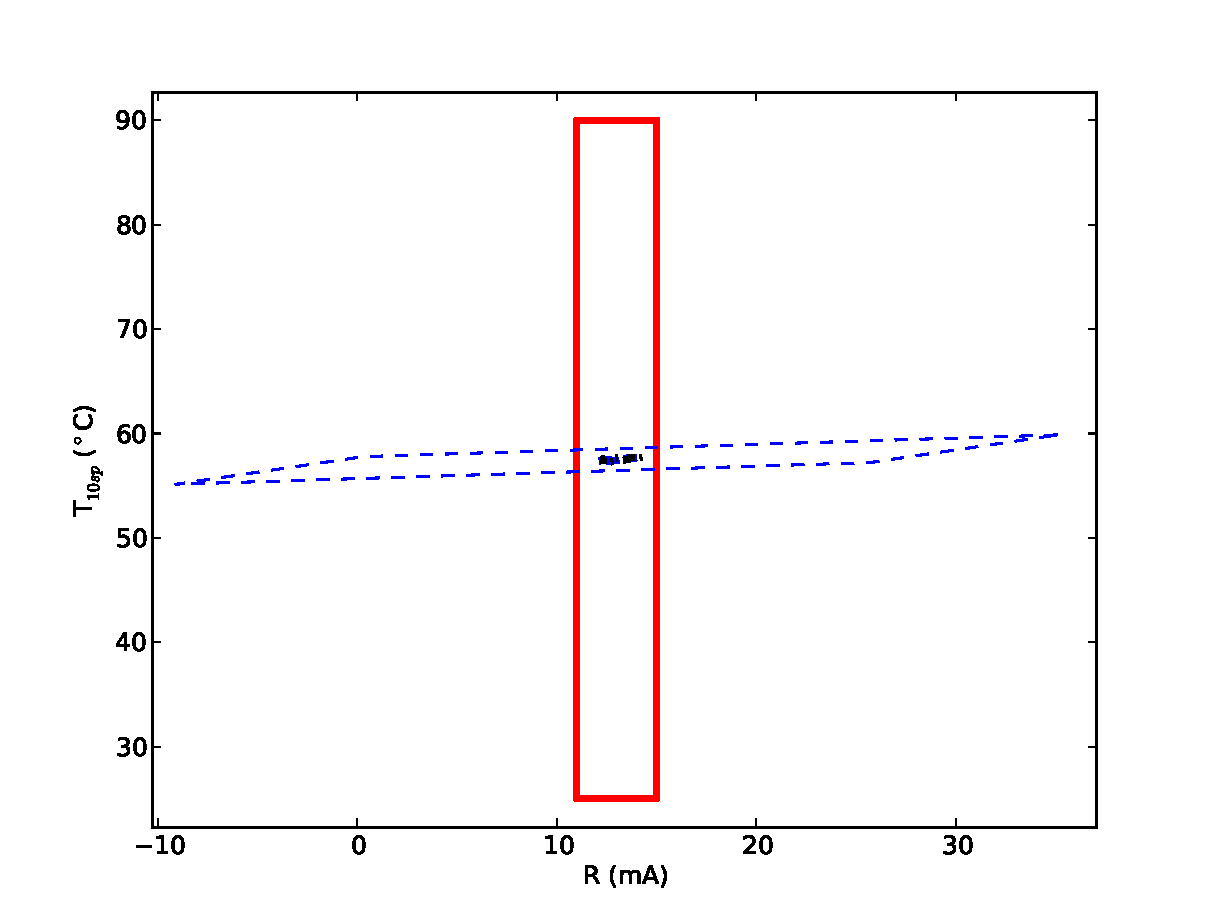
\includegraphics[width=8cm]{columninputs.pdf}
%    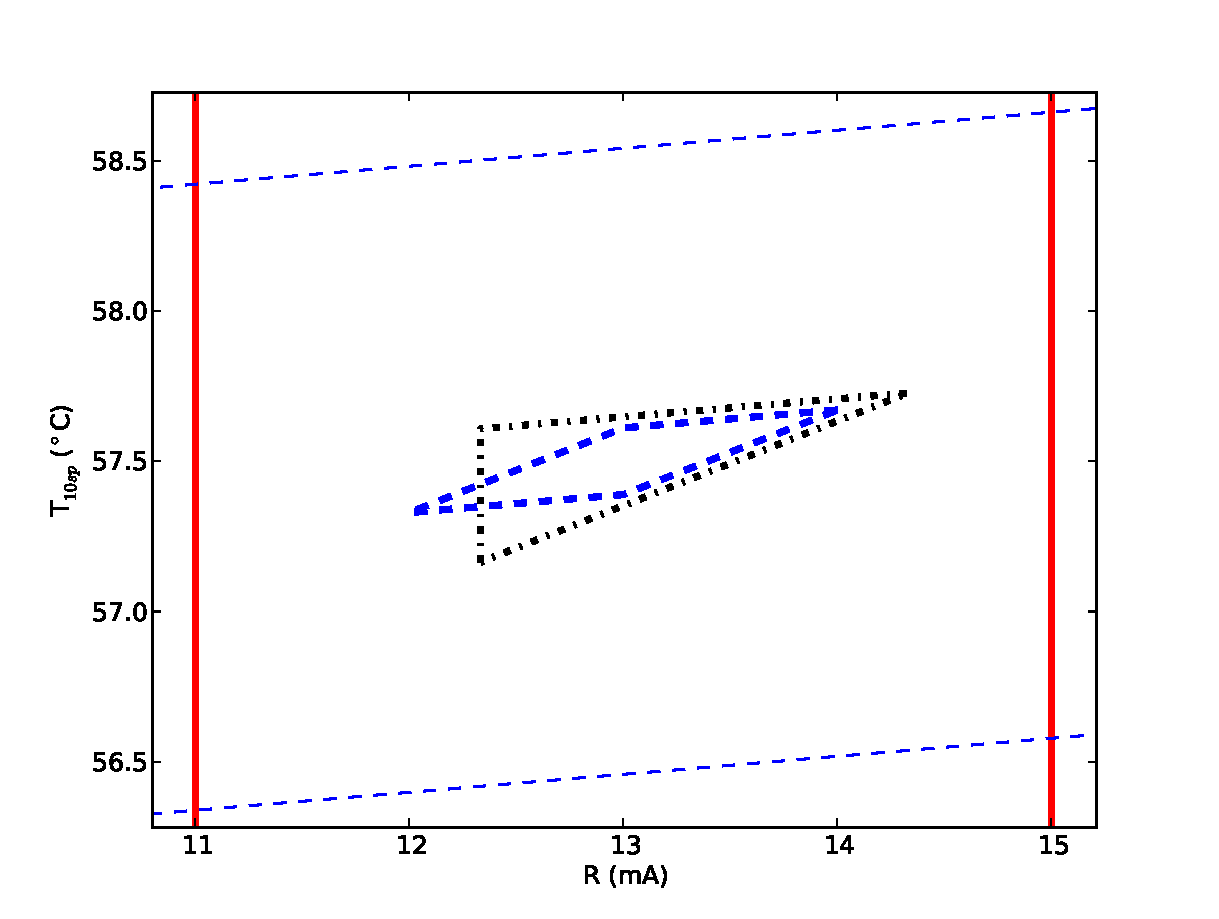
\includegraphics[width=8cm]{columninputszoom.pdf}
    \beginpgfgraphicnamed{figure4b}
    \scalebox{1}{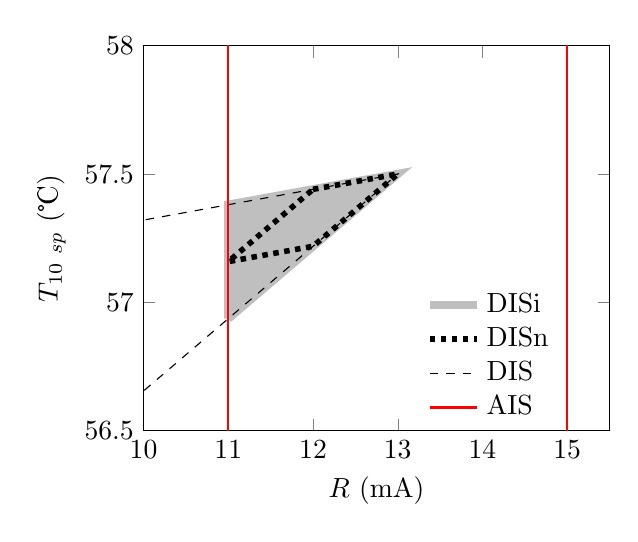
\begin{tikzpicture}
  \begin{axis}[
    width=7.5cm,
    xlabel=$R$~(mA),
    ylabel=$T_{10~sp}$~(\textcelsius),
    xmin=10,xmax=15.5,ymin=56.5,ymax=58,
 %   xtick={67,67.2,...,68.4},
 %   ytick={77.7,77.8,...,78.4},
    legend style={
      draw=none,
      at={(0.9,0.0)},
      anchor=south east,
      cells={anchor=west}}]
    %DISi
    \addplot[fill=lightgray,color=lightgray, line width=3pt] coordinates {
    (10.99999671,  56.93629251)
    (10.99999669,  57.38020814)
    (13.        ,  57.5       )
    (10.99999671,  56.93629251)
    };
    %DISn
    \addplot[color=black,dotted,line width=2pt] coordinates {
    (11.99935592,  57.44006533)
    (12.99999931,  57.49999969)
    (12.00063675,  57.21832608)
    (10.99999337,  57.15839171)
    (11.99935592,  57.44006533)
    };
    %DIS
    \addplot[color=black,dashed] coordinates {
    (-21.79048698,  55.41619479)
    ( 13.        ,  57.5       )
    (  3.61381653,  54.85447339)
    (-31.17667044,  52.77066818)
    (-21.79048698,  55.41619479)
    };
    %AIS
    \addplot[color=red,thick] coordinates {
      (11,25)
      (11,90)
      (15,90)
      (15,25)
      (11,25)
    };
    \legend{DISi,DISn,DIS,AIS}
  \end{axis}
\end{tikzpicture}
}
    \endpgfgraphicnamed
  \caption{Constraints in the input space for the column (a) and focus on the constraint changes showing input clamping (b).}
  \label{fig:columnconsinput}
\end{figure}

Figure~\ref{fig:columnconsinput}(a) also serves to show that the limits of the DOS -- now represented in the input space as the DIS -- are unattainable.

\subsection{Constraint types}
The AIS of the distillation column consists of physical and operational constraints.
The small operating region necessitates the changing of input constraints to increase the process' operability, although the necessary changes are not immediately apparent.
For this reason it is important to identify the constraints that can be changed in the input space (i.e. non-hard, operational constraints) as well as their corresponding constraints in the output space.

The constraints on $R$ (figure~\ref{fig:columnaisaos}(a)) correspond to the long diagonal constraints in the output space (figure~\ref{fig:columnaisaos}(b)).
Therefore, changing the lower bound on $R$ will increase the Operability Index.
Decreasing the lower bound on $R$ to 4~mA increases the Operability Index to 0.125.

This highlights the importance of constraint and model interaction, as changing the limits on $T_{10~sp}$ (if this were possible) would have no effect on the process operability.


\section{Conclusions}\label{sec:conclusions}
From the proposed method of systematic constraint handling and the illustrative example, these conclusions can be drawn:
\begin{itemize}
  \item Checking constraints via the process model can identify constraints which are not attainable and should be revised.
  \item The constraints describing the AOS and DOS intersection represent the largest operating region for the given input and output constraints.
By adding unmeasured variables to the process model, these linear constraints can be reformatted and directly applied in the high and low limit structure of commercial MPC interfaces.
  \item When constraint changes are made (during operation or design), checking changes to constraints via the process model allows for a measure of clamping (or relaxing) to be determined.
This highlights the effect of changing constraints and can guide design or operation decisions.
\end{itemize}

Finally, disambiguating the language used in specifying constraints, allow for identification of constraints that can be adjusted to increase process operability.
In the case of a process still in the design phase, the specific effect of constraints on variables can be used as a guide for possible design modifications. 

%% ==== TAIL ====
\bibliographystyle{model1-num-names}
\bibliography{articlerefs}

\end{document}
